This chapter contains the information regarding the use case regarding contingency analysis. The information is presented visually, grouped in tables and figures for a better comprehension. It has to be mentioned that although the central part of this chapter revolves around the definition of a high level use case, details about the primary use cases are also given. They are partially adapted from the European RESOLVD project \cite{melendez2019resolvd}.

\section{Scope and objectives}
Table \ref{tab:scopee} presents the scope and the objective of the use case.

\begin{table}[!htb]\centering
  \renewcommand{\arraystretch}{1.6}
    \centering
\begin{tabularx}{\linewidth}{|l|L|} 
    \hline
\textbf{Attribute} & \textbf{Description}\\ 
    \hline
\textbf{Scope} & The scope of the UC is to evaluate the effects of a fault and calculate any overloads based on a computer application that simulates the power system to be prepared for any possible fault. \\
\hline
\textbf{Objective} & Prediction of the impact of faults. \\
\hline
\textbf{Related Grid Problems} & Grid faults: \\
                               & \vspace{-0.25cm} \begin{itemize} \item Short-circuits \end{itemize} \\
                               & \vspace{-0.75cm} \begin{itemize} \item Overloads \end{itemize} \\
                               & \vspace{-0.75cm} \begin{itemize} \item Undervoltages \end{itemize} \\
    \hline
\textbf{Relation to other use cases} & \begin{itemize} \item PUC 01: Demand and generation forecasting \end{itemize} \\
                                     & \vspace{-1cm} The EF can predict demand and generation curves at specific points of the grid. \\
                                     & \begin{itemize} \item PUC 02: Grid Operation Scheduling \end{itemize} \\
                                     & \vspace{-1cm} The Grid Operation Scheduler is capable of providing an optimal schedule of the grid to avoid possible faults and allow the continuity of supply. \\
                                     & \begin{itemize} \item PUC 03: Grid observability and monitoring \end{itemize} \\
                                     & \vspace{-1cm} It permits to program a series of alerts for a better monitoring of the overall status of the grid. \\
                                     & \begin{itemize} \item PUC 04: Fault detection and localization \end{itemize} \\
                                     & \vspace{-1cm} The Fault Detection Application analyses data, comparing them with the expected operation conditions to detect possible faults. \\
    \hline
\textbf{Viewpoint} & Technical \\
\hline
\textbf{Type} & HLUC \\
\hline
\end{tabularx}
\caption{Scope and objectives of the contingency analysis use case}
\label{tab:scopee}
    \end{table}

Table \ref{tab:descr} contains the description of the use case.

\begin{table}[!htb]\centering
  \renewcommand{\arraystretch}{2}
  \begin{tabularx}{\linewidth}{|L|}
    \hline
    \textbf{Short description} \\
    \hline
    Using simulation data, demand and generation forecasting and monitoring systems, the contingency analysis is able to detect and locate faults. When faults are located, they alert the operator. Then, the power flow is computed to determine the impact on the system. \\
    \hline
    \textbf{Complete description} \\
    \hline
    Fault detection and data monitoring constantly analyse the system data to detect and then locate faults in the grid. When faults are detected, the operator is notified, in order to start the mitigation process. \\
The process consists of forecasting the energy supply and demand conditions of the grid on one hand; on the other evaluating the consistency of the grid after the impact of a fault. \\
For forecasting energy demand and supply conditions, the energy forecaster performs the forecast using smart meters data stored in the meter data management system and weather forecast data provided by the weather forecaster. This falls somewhat outside the scope of the use case, but the central idea is that these actors provide information related to contingencies which is then further processed. \\
\hline
  \end{tabularx}
  \caption{Narratives of the contingency analysis}
  \label{tab:descr}
\end{table}

\section{Mapping}
After having defined the general view of the use case, more details are given following the SGAM model. First, Figure \ref{fig:comps} shows the component layer.

\begin{figure}[!htb]\centering
  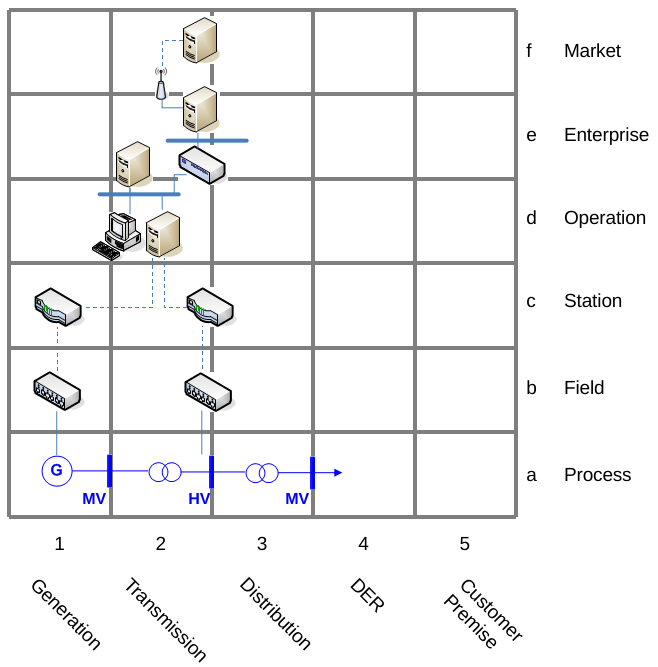
\includegraphics[width=9.5cm]{Data/components.png}
  \hspace{0.3cm}
  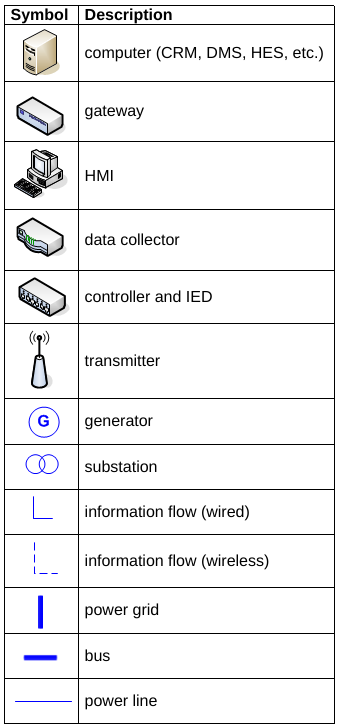
\includegraphics[width=4.4cm]{Data/legends.png}
\caption{Component layer overview and components legend}
\label{fig:comps}
\end{figure}
Components are for the most part placed between transmission and distribution, as they are the domains where contingencies are assumed to be more common and impactful. The central idea is to gather the data from the field and then be able to process it at the upper zones.

Then, Figures \ref{fig:busins} and \ref{fig:functs} present the distribution and links between the several actors that intervene.

\begin{figure}[!htb]\centering
  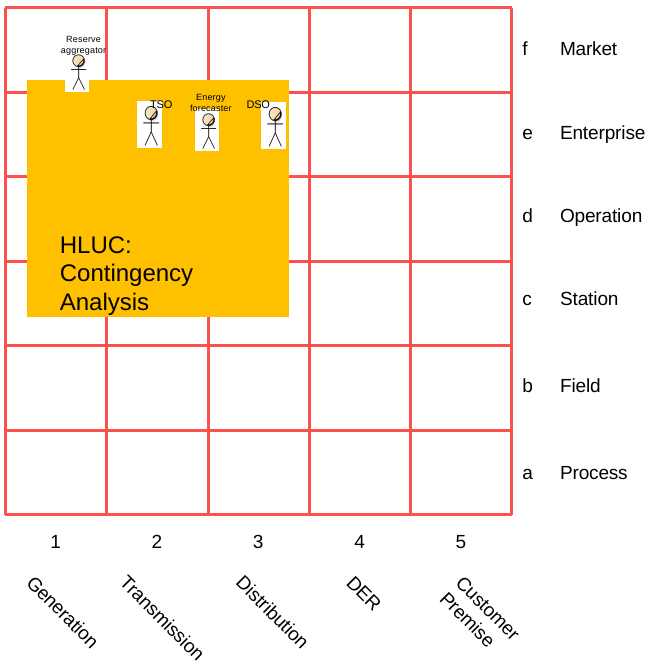
\includegraphics[width=8.0cm]{Data/business.png}
\caption{Business layer mapping}
\label{fig:busins}
\end{figure}


\begin{figure}[!htb]\centering
  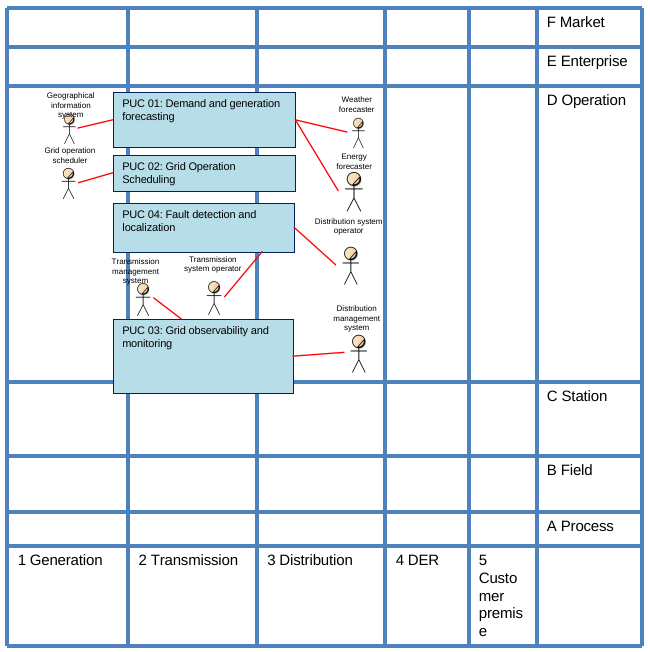
\includegraphics[width=8.0cm]{Data/function.png}
\caption{Function layer mapping}
\label{fig:functs}
\end{figure}

As mentioned before, the actors are generally placed in the generation, transmission and distribution domains. The most relevant zones are the operation, the station and the enterprise. While the operators of the system are the main actors when it comes to business aspects, there are various underlying actors associated to the particular primary use cases (PUC). They several involved PUCs have been exctracted from \cite{melendez2019resolvd}. They are defined for the sake of completeness. 

\subsection{PUC 01: Demand and generation forecasting}


\begin{figure}[!htb]\centering
  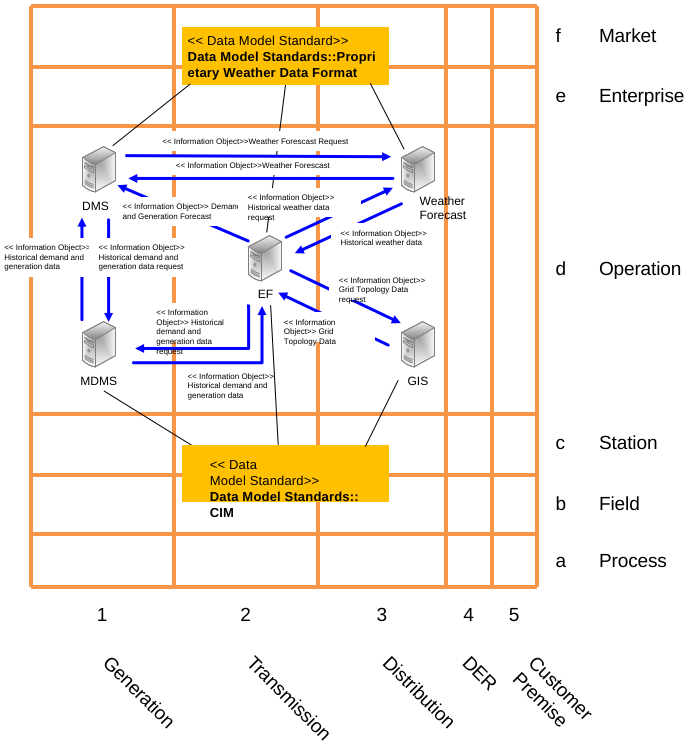
\includegraphics[width=9cm]{Data/i1.png}
\caption{Information layer for PUC 01}
\label{fig:i1}
\end{figure}


\begin{figure}[!htb]\centering
  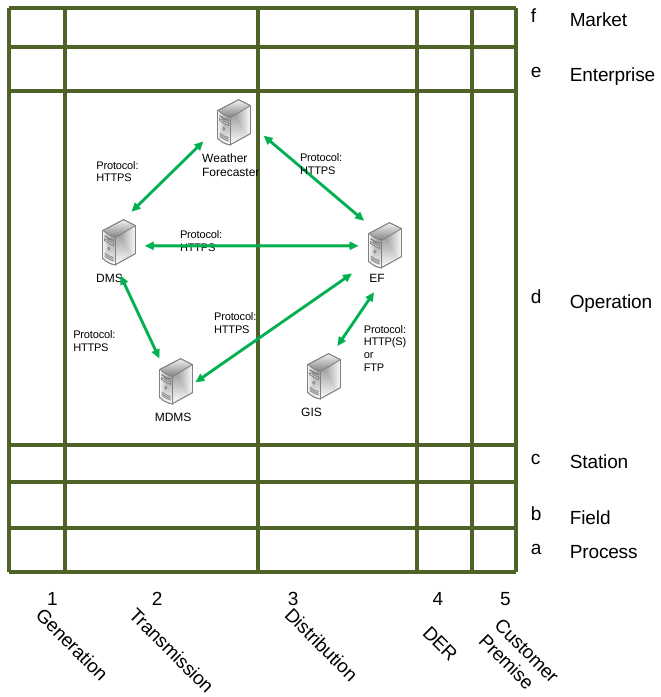
\includegraphics[width=9cm]{Data/c1.png}
\caption{Communication layer for PUC 01}
\label{fig:c1}
\end{figure}






\subsection{PUC 02: Grid Operation Scheduling}


\begin{figure}[!htb]\centering
  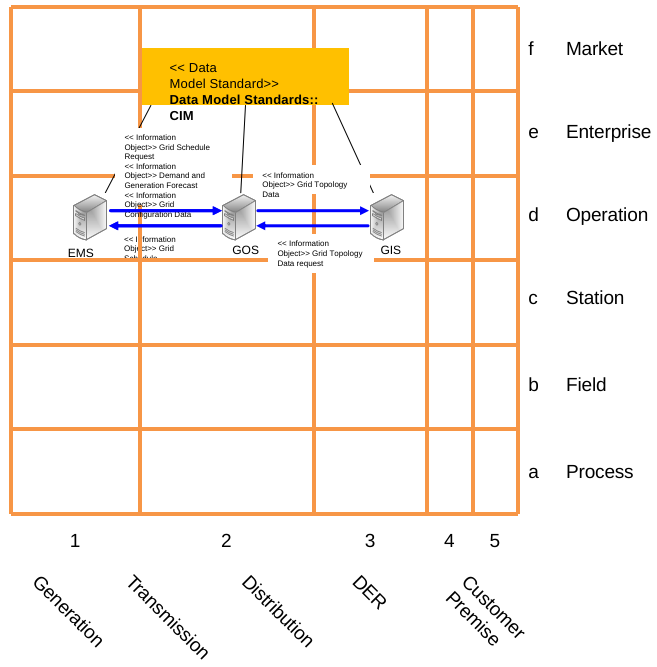
\includegraphics[width=9.0cm]{Data/i2.png}
\caption{Information layer for PUC 02}
\label{fig:i2}
\end{figure}


\begin{figure}[!htb]\centering
  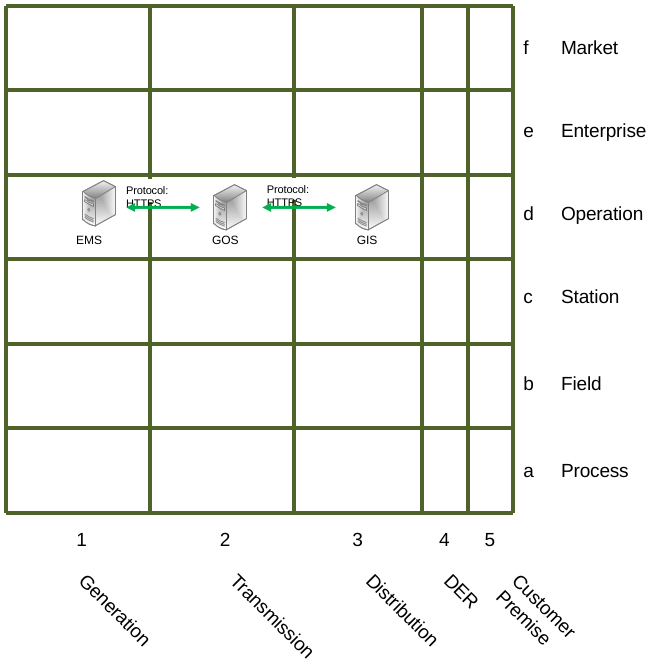
\includegraphics[width=9.0cm]{Data/c2.png}
\caption{Communication layer for PUC 02}
\label{fig:c2}
\end{figure}



\clearpage
\newpage
\subsection{PUC 03: Grid ovservability and monitoring}


\begin{figure}[!htb]\centering
  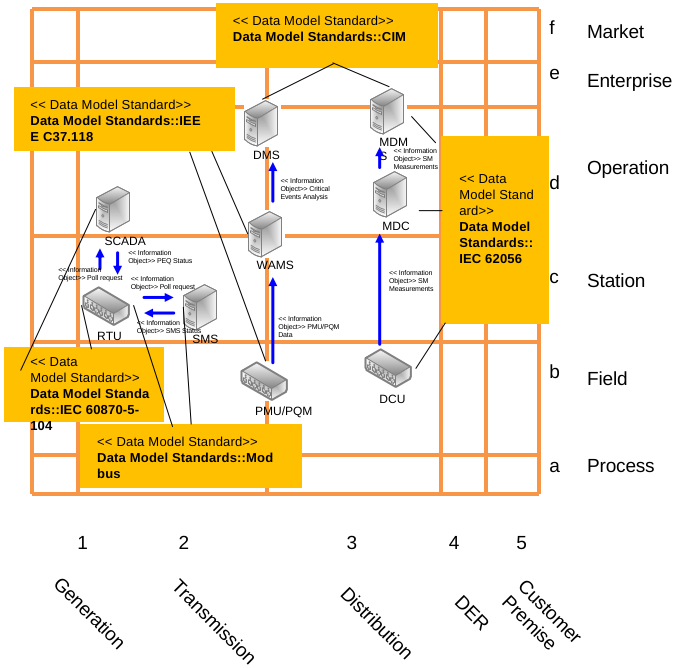
\includegraphics[width=9.0cm]{Data/i3.png}
\caption{Information layer for PUC 03}
\label{fig:i3}
\end{figure}


\begin{figure}[!htb]\centering
  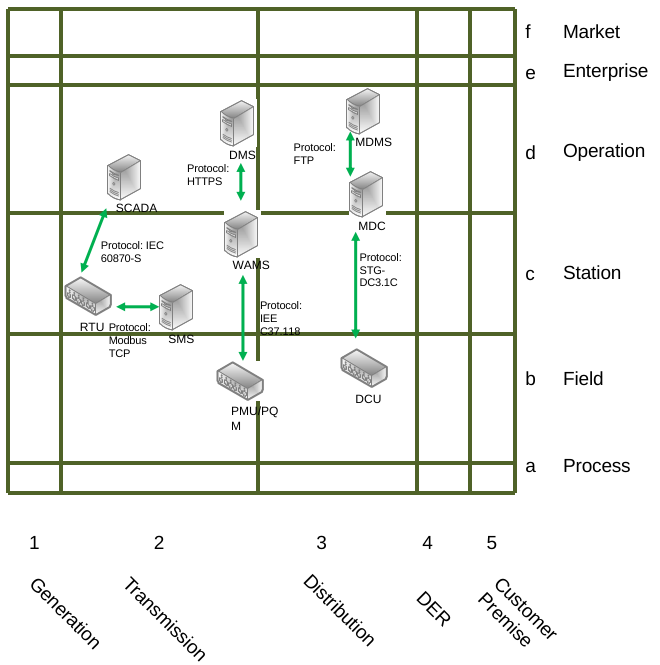
\includegraphics[width=9.0cm]{Data/c3.png}
\caption{Communication layer for PUC 03}
\label{fig:c3}
\end{figure}




\clearpage
\newpage
\subsection{PUC 04: Fault detection and localization}


\begin{figure}[!htb]\centering
  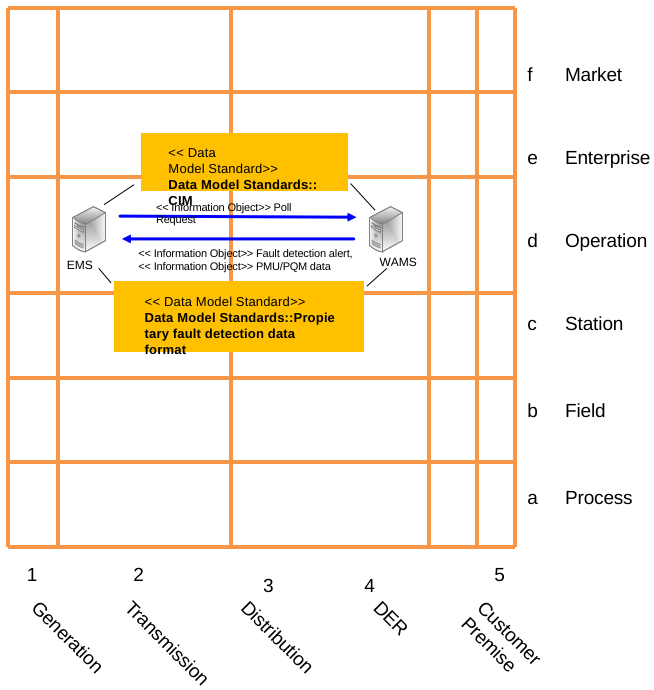
\includegraphics[width=9.5cm]{Data/i4.png}
\caption{Information layer for PUC 04}
\label{fig:i4}
\end{figure}


\begin{figure}[!htb]\centering
  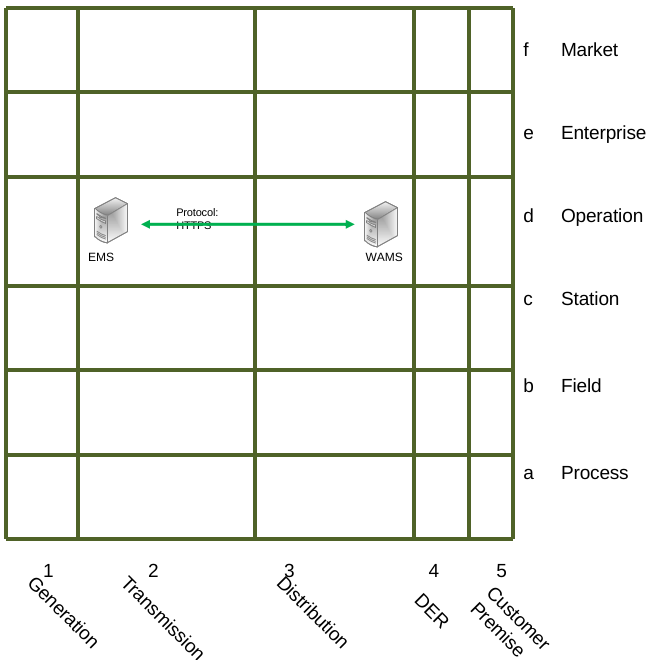
\includegraphics[width=9.5cm]{Data/c4.png}
\caption{Communication layer for PUC 04}
\label{fig:c4}
\end{figure}



